The schematic for the One Evaporator Transcritical Heat Pump cycle (TC1) is shown 
in Figure \ref{fig:TC1} and the corresponding operating conditions are summarized in Table 
\ref{tab:TC1_conditions}.

\begin{figure}[H]
    \centering
    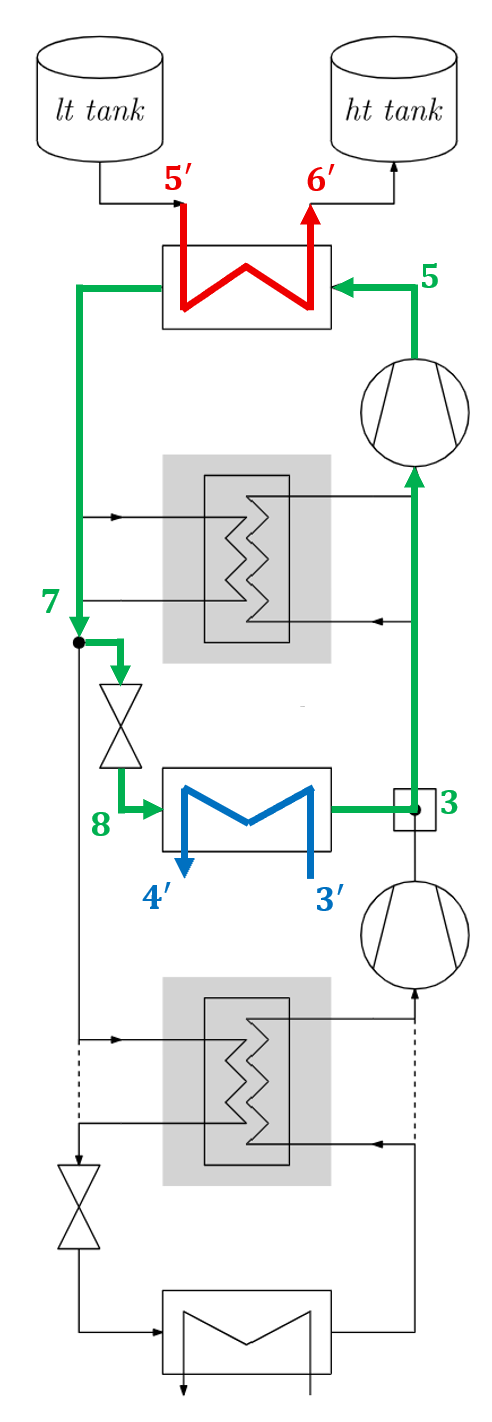
\includegraphics[width=0.35\textwidth]{Figures/TC1.png}
    \begin{minipage}{0.7\textwidth}
        \caption{Schematic of the One Evaporator Transcritical Heat Pump cycle (TC1) 
        (\textit{green: working fluid; blue: heat source(s); red: heat sink})}
        \label{fig:TC1}
    \end{minipage}
\end{figure}

\begin{table}[H]
\centering
\begin{tabular}{|c|c|c|c|}
\hline
 & \textbf{Heat source} & \textbf{Working fluid} & \textbf{Heat sink} \\
\hline
Fluid & Water & R290 (propane) & Water \\
%\hline
Inlet temperature & $T_{3}' = 40\,^{\circ}\mathrm{C}$ & -- & $T_{5}' = 60\,^{\circ}\mathrm{C}$ \\
%\hline
Mass flow rate & $\dot{m}_\mathrm{c} = 0.5\,\mathrm{kg/s}$ & -- & $\dot{m}_\mathrm{h} = 0.1\,\mathrm{kg/s}$ \\
\hline
\end{tabular}
\caption{Operating conditions for the TC1 cycle}
\label{tab:TC1_conditions}
\end{table}

%\textbf{Note:} The heat sink mass flow rate is lower than 
%in the SC2 cycle to increase the temperature glide, 
%as transcritical cycles generally perform better with 
%larger temperature differences compared to subcritical cycles.
\newpage